% !TEX encoding = UTF-8 Unicode
\documentclass[14pt,a4paper]{article}

\usepackage{lipsum}
\usepackage[margin=2cm,includefoot]{geometry}
\usepackage[utf8]{inputenc}
\usepackage[russian]{babel}
\usepackage{amssymb}
\usepackage{amsmath}
\usepackage{amsthm}
\usepackage{latexsym}
\usepackage{dsfont}
\usepackage[linesnumbered]{algorithm2e}
\usepackage{mathtools}
\usepackage{indentfirst}
\usepackage{listings}

\usepackage{tikz} 
\usepackage{tikz-qtree}

\usepackage{graphicx}
\usepackage{float}
\graphicspath{ {./} }

\usepackage{tabularx}
\usepackage{makecell}
\usepackage{multirow}

\newcolumntype{q}{>{\hsize=.4\hsize}X}
\newcolumntype{w}{>{\hsize=1.6\hsize}X}
\newcolumntype{e}{>{\hsize=.25\hsize}X}

\usepackage{titling}
\renewcommand\maketitlehooka{\null\mbox{}\vfill}
\renewcommand\maketitlehookd{\vfill\null}

%\DeclarePairedDelimiter\ceil{\lceil}{\rceil}
%\DeclarePairedDelimiter\floor{\lfloor}{\rfloor}

%\def\changemargin#1#2{\list{}{\rightmargin#2\leftmargin#1}\item[]}
%\let\endchangemargin=\endlist 

%\newcommand\tab[1][0.7cm]{\hspace*{#1}}

%\newcommand{\hm}[1]{#1\nobreak\discretionary{}{\hbox{\ensuremath{#1}}}{}}

%\renewcommand*{\qed}{\hfill\ensuremath{\blacksquare}}%

\usepackage{fancyhdr}
\pagestyle{fancy}
\thispagestyle{empty}
\fancyhead{}
\fancyfoot{}
\fancyfoot[R]{ \thepage\ }
\renewcommand{\headrulewidth}{0pt}
\renewcommand{\footrulewidth}{1pt}

\usepackage{hyperref}
\hypersetup{
    colorlinks=false, %set true if you want colored links
    linktoc=all,     %set to all if you want both sections and subsections linked
    %linkcolor=blue,  %choose some color if you want links to stand out
}

\begin{document}

\text{}
\vskip 8cm
\begin{center}
\begin{minipage}{0.8\textwidth}
\begin{center}
\Huge Веб-приложение для распознавания музыкальных инструментов и преобразования аудиозаписей
\end{center}
\end{minipage}
\end{center}

\vskip 5.5cm

\begin{flushright}
\Large \underline{Авторы}: \\
Бухараев Алим \\
Прохоров Юрий \\
Савелов Михаил \\
Яушев Фарух \\
\bigskip
\Large \underline{Руководитель}: \\
Бабичев Сергей Леонидович
\end{flushright}

\vskip 2.6cm

\begin{center}
2019
\end{center}

\newpage

\renewcommand\contentsname{\huge Содержание}
\setcounter{tocdepth}{2}
\Large \tableofcontents
\normalsize

\newpage 

\section[Техническое задание]{\huge Техническое задание}

\subsection{Аннотация}

Данный проект --- курсовая работа вышеперечисленных студентов второго курса ФУПМ (факультета управления и прикладной математики) МФТИ. Он состоит из 3 основных обособленных частей:
\begin{enumerate}
\item Библиотека и API на C++ для обработки аудиозаписей.
\item API в виде расширения PHP для обработки аудиозаписей.
\item Пользовательский интерфейс в виде веб-приложения.
\end{enumerate}
Об установке можно прочитать ниже. Ссылка на репозиторию Github:\\\\
\makebox[\textwidth][c]{
   \fbox{\begin{minipage}{10cm}
\centering \url{https://github.com/suchusername/sounds}
\end{minipage}}}\\

Изначально, у нас была идея написать программу, способную распознавать музыкальные инструменты на аудиозаписи. Причина связана с тем, что эта задача не имеет точных результатов, и мы хотели получить свое собственное частное решение. Затем мы решили расширить функционал нашего приложения, добавив наиболее популярные запросы, и реализовать его как легко доступный пользователю веб-сервис. Таким образом, основные цели проекта:
\begin{itemize}
\item Повышение командных навыков.
\item Реализация приложения по популярной тематике.
\item Применение знаний языка C++.
\item Изучение новых инструментов и технологий.
\end{itemize}

Пользователю предлагается загрузить свой файл в формате WAV на сервер. После этого он получает некоторую статистику о файле и выбирает, какое действие он желает выполнить с ним или сразу с несколькими файлами. Среди возможных функций: предсказание музыкального инструмента по аудиозаписи, слияние файлов, их обрезка, усиление громкости, ускорение и другие преобразования. Аудиозапись хорошего качества может быть использована далее для дальнейшего обучения нашей или каких-либо других моделей. Наконец, преобразованный файл пользователь может прослушать и загрузить обратно на свое устройство.\\

При разработке приложения использовались следующие технологии:
\begin{itemize}
\item Язык С++ стандарта 11 для написания серверной составляющей (ядра).
\item Набор инструментов для написания расширения PHP на С++.
\item Python 3 и библиотеки Keras, NumPy, SciPy для реализации нейронной сети.
\item Средства PHP, HTML5, CSS и Javascript для разработки пользовательского интерфейса.
\end{itemize}

\subsection{Цели}

Главной мотивацией работы является его выполнение в качестве курсового проекта по информатике студентов второго курса ФУПМ МФТИ: Бухараева Алима, Прохорова Юрия, Савелова Михаила и Яушева Фаруха. Руководитель проекта --- Бабичев Сергей Леонидович. \\

Другая важная цель --- реализация классификатора мелодий по играющему музыкальному инструменту. Нами был проведен анализ уже существующих средств распознавания музыкальных инструментов, и, как оказалось, тема не является очень популярной. Мы же считаем, что данный этап предобработки аудиозаписей принесет большую пользу для дальнейшего их анализа (например, распознавания играющей композиции, удаления некоторых тональностей или инструментов), поэтому мы попробовали внести свой вклад в решение данной задачи. \\

Еще одна задача проекта --- это разработка доступного пользовательского интерфейса для простейшей обработки аудиофайлов. Мы не нашли сайта, который представляет собой ''онлайн-редактор аудиозаписей'', и в связи с этим решили дополнить нашу программу этими функциями и предоставить ее как веб-сервис. \\

Наконец, важной для нас целью является обретение опыта работы в команде и грамотное распределение обязанностей. Кроме того, сюда же входит получение опыта приложения полученных знаний о языке C++ к реальной задаче, изучение новых полезных для практического применения технологий и инструментов.

\subsection{Требования}

В данном разделе перечислены все задачи и подзадачи, которые мы поставили перед собой в рамках выполнения настоящей проектной работы.

\begin{enumerate}
\item Библиотека и API на C++.
    \begin{itemize}
    \item Разработка объектно-ориентированной внутренней структуры библиотеки.
    \item Побайтовый разбор файла формата WAV.
    \item Реализация функционала
        \begin{itemize}
        \item[--] Вывод статистики о файле.
        \item[--] Изменение громкости.
        \item[--] Ускорение аудиозаписи.
        \item[--] Слияние аудиозаписей.
        \item[--] Предсказание музыкального инструмента.
        \item[--] Обрезка аудизаписи.
        \end{itemize}
    \item Универсальный пользовательский интерфейс с вышеперечисленными функциями.
    \end{itemize}
\item Нейронная сеть.
    \begin{itemize}
    \item Подготовка и нарезка датасета для обучения модели. 
    \item Поиск оптимального способа предобработки аудиозаписей.
    \item Моделирование наиболее эффективной архитектуры классификатора, различающего музыкальные инструменты.
    \item Обучение классификатора на подготовленных данных.
    \item Анализ результатов.
    \end{itemize}
\item Расширение PHP.
    \begin{itemize}
    \item Настройка Apache веб-сервера и установка необходимых инструментов для реализации PHP-расширения.
    \item Универсальный пользовательский интерфейс с вышеперечисленными функциями.
    \end{itemize}
\item Веб-приложение.
    \begin{itemize}
    \item Загрузка нескольких файлов одновременно.
    \item Выбор файла/файлов, которые требуется преобразовать.
    \item Просмотр статистики об аудиозаписи.
    \item Загрузка файла с сервера обратно.
    \end{itemize}
\end{enumerate}

\subsection{Распределение обязанностей}

\begin{table}[H]
\begin{tabularx}{\textwidth}{qw}
\hline
\multicolumn{1}{|c|}{Член команды} & \multicolumn{1}{c|}{Задача}  \\ \hline
 &   \\ \hline
\multicolumn{1}{|c|}{\multirow{5}{*}{Бухараев Алим}} & \multicolumn{1}{c|}{Изучение сверточных и рекуррентных нейронных сетей} \\ \cline{2-2} 
\multicolumn{1}{|c|}{} & \multicolumn{1}{c|}{\makecell{Поиск большого числа мелодий, пригодных для использования \\ в качестве обучающей выборки}} \\ \cline{2-2} 
\multicolumn{1}{|c|}{} & \multicolumn{1}{c|}{Проектирование и обучение модели-классификатора} \\ \cline{2-2} 
\multicolumn{1}{|c|}{} & \multicolumn{1}{c|}{Подготовка презентации} \\ \hline
 &   \\ \hline
\multicolumn{1}{|c|}{\multirow{4}{*}{Прохоров Юрий}} & \multicolumn{1}{c|}{Реализация анализатора файла формата .WAV} \\ \cline{2-2} 
\multicolumn{1}{|c|}{} & \multicolumn{1}{c|}{Различные преобразования аудиозаписей и реализация библиотеки C++} \\ \cline{2-2} 
\multicolumn{1}{|c|}{} & \multicolumn{1}{c|}{Реализация программного интерфейса расширения PHP} \\ \cline{2-2} 
\multicolumn{1}{|c|}{} & \multicolumn{1}{c|}{Написание отчета и документации}\\ \hline
  &  \\ \hline
\multicolumn{1}{|c|}{\multirow{4}{*}{Савелов Михаил}} & \multicolumn{1}{c|}{Изучение PHP, HTML5, JavaScript и CSS} \\ \cline{2-2} 
\multicolumn{1}{|c|}{} & \multicolumn{1}{c|}{Моделирование пользовательского интерфейса} \\ \cline{2-2} 
\multicolumn{1}{|c|}{} & \multicolumn{1}{c|}{Разработка структуры веб-страницы}  \\ \cline{2-2} 
\multicolumn{1}{|c|}{} & \multicolumn{1}{c|}{Дизайн} \\ \hline 
  &  \\ \hline
\multicolumn{1}{|c|}{\multirow{4}{*}{Яушев Фарух}} & \multicolumn{1}{c|}{Изучение PHP, HTML5, JavaScript и CSS} \\ \cline{2-2} 
\multicolumn{1}{|c|}{} & \multicolumn{1}{c|}{Моделирование пользовательского интерфейса} \\ \cline{2-2} 
\multicolumn{1}{|c|}{} & \multicolumn{1}{c|}{Разработка структуры веб-страницы}  \\ \cline{2-2} 
\multicolumn{1}{|c|}{} & \multicolumn{1}{c|}{Дизайн} \\ \hline 
\end{tabularx}
\end{table}

\newpage

\section[Документация]{\huge Документация}
\subsection{Структура директорий в репозитории}

В этом и следующем разделах приведено описание репозитории проекта на GitHub.

\subsubsection*{Audios}

В данную директорию загружаются все пользовательские файлы, там же создаются новые промежуточные аудиофайлы.

\subsubsection*{Classes}

В этой директории находятся реализации методов всех классов на C++. Каждому классу соответствует свой файл. Классы, отвечающие преобразованиям аудиозаписей вынесены в отдельную папку \textit{Classes/Queries}.

\subsubsection*{Documentation}

В этой директории находится данный документ и его .tex файл. Также в папке \textit{Documentation/Papers} присутствуют статьи на разные тематики, которые использовались при написании этой проектной работы.

\subsubsection*{Instrument\_classifier}
\lstset{
  language=bash,
  basicstyle=\ttfamily
}

В этой директории находятся следующие файлы:
\begin{itemize}
\item \textit{launch.py} \\
Содержит реализацию нейронной сети с использованием библиотеки Keras. Этот же файл отвечает за получения предсказания на конкретной аудиозаписи. Нейронную сеть можно явно использовать следующим образом:
\begin{lstlisting}
cd Instrument_classifier
python3 launch.py path/to/file.wav
\end{lstlisting}
\item \textit{my\_model\_$\ast$.h5} \\
Различные версии модели.
\end{itemize}

\subsubsection*{root}

Данная директория является корневой директорией Apache веб-сервера. В ней содержатся следующие объекты:
\begin{itemize}
\item \textit{$\ast$.php} \\
Файлы формата .php --- ответы сервера на запросы клиента. Они генерируют html код, который видит пользователь.
\item \textit{sounds\_update.sh} \\
Shell-скрипт, который делает новую сборку расширения PHP, переустанавливает его и перезапускает Apache веб-сервер.
\item \textit{logs} \\
Текстовый файл с отладочной информацией.
\item \textit{root/css, root/js} \\
Эти папки содержат файлы соответствующего формата, необходимые для реализации дизайна и пользовательского интерфейса веб-страницы.
\item \textit{root/sounds} \\
Эта папка содержит все файлы, необходимые для создания расширения PHP. Среди них:
    \begin{itemize}
    \item[--] \textit{config.m4} \\
    Файл c параметрами для компилиции расширения PHP.
    \item[--] \textit{php\_sounds.h} \\
    Задание интерфейса PHP-расширения.
    \item[--] \textit{sounds.cc} \\
    Реализация методов PHP-расширения.
    \end{itemize}
\end{itemize}

\subsection{Конкретные файлы в репозитории}

\subsubsection*{config.h}

В этом файле содержатся все константы, используемые во всех файлах.

\subsubsection*{server.h}

В этом файле содержится объявление всех классов и их методов. Также там присутствует описания функций программного интерфейса.

\subsubsection*{sounds\_cpp\_api.cc}

Реализация методов программного интерфейса.

\subsubsection*{main.cc}

Этот файл предназначен только для тестирования различных функций.

\subsection{Документация: библиотека C++}

\lstset{
  language=C++,
  backgroundcolor=\color{black!5},
  keywordstyle=\color{blue},
  basicstyle=\ttfamily
}

В этом разделе перечислен весь функционал библиотеки с указаниями, как им пользоваться. Также к некоторым методам приведены примеры использования.

\subsubsection*{Информация об аудиозаписи}

\begin{lstlisting}
vector<double> sounds_info(const string &name);
\end{lstlisting}

\lstinline{name} --- полный путь к файлу относительно текущей директории. \\

\noindent Возвращает вектор из $6$ элементов:
\smallskip 
\begin{itemize}
\item[] \lstinline{[0]} --- Размер файла в байтах.
\item[] \lstinline{[1]} --- Число аудиоканалов ($1$ --- моно, $2$ --- стерео).
\item[] \lstinline{[2]} --- Sample rate (количество значений амплитуды каждую секунду), обычно $44100$.
\item[] \lstinline{[3]} --- Bit depth (число битов на каждый sample).
\item[] \lstinline{[4]} --- Количество sample'ов в аудиофайле.
\item[] \lstinline{[5]} --- Продолжительность аудиофайла (в секундах).
\end{itemize}

\noindent Если элемент вектора \lstinline{[0]} $= -1$, то ошибка.

\subsubsection*{Распознавание музыкальных инструментов}

\begin{lstlisting}
vector<double> sounds_classify(const string &name);
\end{lstlisting}

\lstinline{name} --- полный путь к файлу относительно текущей директории. \\

\noindent Возвращает вектор из $5$ элементов с вероятностями музыкальных инструментов:
\smallskip 
\begin{itemize}
\item[] \lstinline{[0]} --- аккордион
\item[] \lstinline{[1]} --- пианино
\item[] \lstinline{[2]} --- скрипка
\item[] \lstinline{[3]} --- гитара
\item[] \lstinline{[4]} --- флейта
\end{itemize}

\noindent Если элемент вектора \lstinline{[0]} $= -1$, то ошибка.

\subsubsection*{Обрезка аудиозаписей}

\begin{lstlisting}
string sounds_crop(const string &name, const string &new_name, 
	double left = 0, double right = -1);
\end{lstlisting}

\lstinline{name} --- полный путь к файлу относительно текущей директории \par
\lstinline{new_name} --- полный путь c новым названием преобразованного файла \par
\lstinline{left = 0} --- левая граница обрезки в миллисекундах (default: начало файла) \par
\lstinline{right = -1} --- правая граница обрезки в миллисекундах (default: конец файла) \\

\noindent Если \lstinline{left} $\leq 0$ или $\geq$ длины файла, то левая граница --- начало файла. Если \lstinline{right} $\leq 0$ или $\geq$ длины файла, то правая граница --- конец файла. По умолчанию, границы --- начало и конец файла соответственно. \\\\
Обрезает аудиозапись и сохраняет ее в указанную директорию под выбранным пользователем именем. \\\\
Возвращает строку:
\smallskip
\begin{itemize}
\item \lstinline{"OK"} --- успешно
\item \lstinline{string} --- строка с текстом ошибки, если неуспешно
\end{itemize}

\subsubsection*{Изменение громкости}

\begin{lstlisting}
string sounds_volume(const string &name, const string &new_name, 
	double k, double left = 0, double right = -1, bool smooth = false);
\end{lstlisting}

\lstinline{name} --- полный путь к файлу относительно текущей директории \par
\lstinline{new_name} --- полный путь c новым названием преобразованного файла \par
\lstinline{k} --- множитель громкости ($0$ --- тишина, $1$ --- без изменений)\par
\lstinline{left = 0} --- левая граница в миллисекундах (default: начало файла) \par
\lstinline{right = -1} --- правая граница в миллисекундах (default: конец файла) \par
\lstinline{smooth = false} --- плавное изменение громкости (линейное, в течение $2$ секунд) \\

\noindent Если \lstinline{left} $\leq 0$ или $\geq$ длины файла, то левая граница --- начало файла. Если \lstinline{right} $\leq 0$ или $\geq$ длины файла, то правая граница --- конец файла. По умолчанию, границы --- начало и конец файла соответственно. \\\\
Если \lstinline{k} $< 0$, то ошибка, если \lstinline{k} $= 0$, то тишина, если $0 <$ \lstinline{k} $< 1$, то аудиозапись становится тише, если \lstinline{k} $> 1$, то аудиозапись становится громче. \textbf{Внимание:} если выбрать \lstinline{k} очень большим (обычно $\sim 5$), то для нормального звучания не хватает битовой глубины, и звук становится обрывистым (что иногда звучит забавно).\\\\
Изменяет громкость выбранного отрезка аудиозаписи и сохраняет ее в указанную директорию под выбранным пользователем именем. \\\\
Возвращает строку:
\smallskip
\begin{itemize}
\item \lstinline{"OK"} --- успешно
\item \lstinline{string} --- строка с текстом ошибки, если неуспешно
\end{itemize}

\subsubsection*{Изменение скорости аудиозаписи}

\begin{lstlisting}
string sounds_speed(const string &name, const string &new_name, 
	double mult);
\end{lstlisting}

\lstinline{name} --- полный путь к файлу относительно текущей директории \par
\lstinline{new_name} --- полный путь c новым названием преобразованного файла \par
\lstinline{mult} --- множитель скорость аудиозаписи ($1$ --- без изменений) \\

\noindent Если \lstinline{mult} $= 0$, то ошибка. Если $0 <$ \lstinline{mult} $< 1$, то аудиозапись становится медленнее в \lstinline{1/mult} раз. Если \lstinline{mult} $= 1$, то без изменений. Если \lstinline{mult} $> 1$, то аудиозапись ускоряется в \lstinline{mult} раз. Если \lstinline{mult} $< 0$, то аудиозапись проигрывается в обратную сторону (инвертируется).\\\\
Изменяет скорость аудиозаписи и сохраняет ее в указанную директорию под выбранным пользователем именем. \\\\
Возвращает строку:
\smallskip
\begin{itemize}
\item \lstinline{"OK"} --- успешно
\item \lstinline{string} --- строка с текстом ошибки, если неуспешно
\end{itemize}

\subsubsection*{Слияние аудиозаписей}

\begin{lstlisting}
string sounds_merge(const string &left, const string &right, 
	const string &new_name);
\end{lstlisting}

\lstinline{left} --- полный путь к первому файлу относительно текущей директории \par
\lstinline{right} --- полный путь ко второму файлу \par
\lstinline{new_name} --- полный путь c новым названием преобразованного файла \\

\noindent Сливает две аудиозаписи в одну и сохраняет ее в указанную директорию под выбранным пользователем именем. \\\\
Возвращает строку:
\smallskip
\begin{itemize}
\item \lstinline{"OK"} --- успешно
\item \lstinline{string} --- строка с текстом ошибки, если неуспешно
\end{itemize}

\subsection{Документация: расширение PHP}

\lstset{
  language=PHP,
  backgroundcolor=\color{green!10},
  keywordstyle=\color{green},
  basicstyle=\ttfamily
}

В этом разделе перечислен весь функционал расширения PHP с указаниями, как им пользоваться. Также к некоторым методам приведены примеры использования. Здесь написано то же самое, что и в разделе по библиотеку C++, но в терминах PHP.

\subsubsection*{Информация об аудиозаписи}

\begin{lstlisting}
sounds_info($name);
\end{lstlisting}

\lstinline{name} --- полный путь к файлу относительно текущей директории. \\

\noindent Возвращает массив из $6$ элементов:
\smallskip 
\begin{itemize}
\item[] \lstinline{[0]} --- Размер файла в байтах.
\item[] \lstinline{[1]} --- Число аудиоканалов ($1$ --- моно, $2$ --- стерео).
\item[] \lstinline{[2]} --- Sample rate (количество значений амплитуды каждую секунду), обычно $44100$.
\item[] \lstinline{[3]} --- Bit depth (число битов на каждый sample).
\item[] \lstinline{[4]} --- Количество sample'ов в аудиофайле.
\item[] \lstinline{[5]} --- Продолжительность аудиофайла (в секундах).
\end{itemize}

\noindent Если элемент массива \lstinline{[0]} $= -1$, то ошибка.

\subsubsection*{Распознавание музыкальных инструментов}

\begin{lstlisting}
sounds_classify($name);
\end{lstlisting}

\lstinline{name} --- полный путь к файлу относительно текущей директории. \\

\noindent Возвращает массив из $5$ элементов с вероятностями музыкальных инструментов:
\smallskip 
\begin{itemize}
\item[] \lstinline{[0]} --- аккордион
\item[] \lstinline{[1]} --- пианино
\item[] \lstinline{[2]} --- скрипка
\item[] \lstinline{[3]} --- гитара
\item[] \lstinline{[4]} --- флейта
\end{itemize}

\noindent Если элемент массива \lstinline{[0]} $= -1$, то ошибка.

\subsubsection*{Обрезка аудиозаписей}

\begin{lstlisting}
sounds_crop($name, $new_name, $left = 0, $right = -1);
\end{lstlisting}

\lstinline{name} --- полный путь к файлу относительно текущей директории \par
\lstinline{new_name} --- полный путь c новым названием преобразованного файла \par
\lstinline{left = 0} --- левая граница обрезки в миллисекундах (default: начало файла) \par
\lstinline{right = -1} --- правая граница обрезки в миллисекундах (default: конец файла) \\

\noindent Если \lstinline{left} $\leq 0$ или $\geq$ длины файла, то левая граница --- начало файла. Если \lstinline{right} $\leq 0$ или $\geq$ длины файла, то правая граница --- конец файла. По умолчанию, границы --- начало и конец файла соответственно. \\\\
Обрезает аудиозапись и сохраняет ее в указанную директорию под выбранным пользователем именем. \\\\
Возвращает строку:
\smallskip
\begin{itemize}
\item \lstinline{"OK"} --- успешно
\item \lstinline{string} --- строка с текстом ошибки, если неуспешно
\end{itemize}

\subsubsection*{Изменение громкости}

\begin{lstlisting}
sounds_volume($name, $new_name, $k, $left = 0, $right = -1, $smooth = False);
\end{lstlisting}

\lstinline{name} --- полный путь к файлу относительно текущей директории \par
\lstinline{new_name} --- полный путь c новым названием преобразованного файла \par
\lstinline{k} --- множитель громкости ($0$ --- тишина, $1$ --- без изменений)\par
\lstinline{left = 0} --- левая граница в миллисекундах (default: начало файла) \par
\lstinline{right = -1} --- правая граница в миллисекундах (default: конец файла) \par
\lstinline{smooth = False} --- плавное изменение громкости (линейное, в течение $2$ секунд) \\

\noindent Если \lstinline{left} $\leq 0$ или $\geq$ длины файла, то левая граница --- начало файла. Если \lstinline{right} $\leq 0$ или $\geq$ длины файла, то правая граница --- конец файла. По умолчанию, границы --- начало и конец файла соответственно. \\\\
Если \lstinline{k} $< 0$, то ошибка, если \lstinline{k} $= 0$, то тишина, если $0 <$ \lstinline{k} $< 1$, то аудиозапись становится тише, если \lstinline{k} $> 1$, то аудиозапись становится громче. \textbf{Внимание:} если выбрать \lstinline{k} очень большим (обычно $\sim 5$), то для нормального звучания не хватает битовой глубины, и звук становится обрывистым (что иногда звучит забавно).\\\\
Изменяет громкость выбранного отрезка аудиозаписи и сохраняет ее в указанную директорию под выбранным пользователем именем. \\\\
Возвращает строку:
\smallskip
\begin{itemize}
\item \lstinline{"OK"} --- успешно
\item \lstinline{string} --- строка с текстом ошибки, если неуспешно
\end{itemize}

\subsubsection*{Изменение скорости аудиозаписи}

\begin{lstlisting}
sounds_speed($name, $new_name, $mult);
\end{lstlisting}

\lstinline{name} --- полный путь к файлу относительно текущей директории \par
\lstinline{new_name} --- полный путь c новым названием преобразованного файла \par
\lstinline{mult} --- множитель скорость аудиозаписи ($1$ --- без изменений) \\

\noindent Если \lstinline{mult} $= 0$, то ошибка. Если $0 <$ \lstinline{mult} $< 1$, то аудиозапись становится медленнее в \lstinline{1/mult} раз. Если \lstinline{mult} $= 1$, то без изменений. Если \lstinline{mult} $> 1$, то аудиозапись ускоряется в \lstinline{mult} раз. Если \lstinline{mult} $< 0$, то аудиозапись проигрывается в обратную сторону (инвертируется).\\\\
Изменяет скорость аудиозаписи и сохраняет ее в указанную директорию под выбранным пользователем именем. \\\\
Возвращает строку:
\smallskip
\begin{itemize}
\item \lstinline{"OK"} --- успешно
\item \lstinline{string} --- строка с текстом ошибки, если неуспешно
\end{itemize}

\subsubsection*{Слияние аудиозаписей}

\begin{lstlisting}
sounds_merge($left, $right, $new_name);
\end{lstlisting}

\lstinline{left} --- полный путь к первому файлу относительно текущей директории \par
\lstinline{right} --- полный путь ко второму файлу \par
\lstinline{new_name} --- полный путь c новым названием преобразованного файла \\

\noindent Сливает две аудиозаписи в одну и сохраняет ее в указанную директорию под выбранным пользователем именем. \\\\
Возвращает строку:
\smallskip
\begin{itemize}
\item \lstinline{"OK"} --- успешно
\item \lstinline{string} --- строка с текстом ошибки, если неуспешно
\end{itemize}

\newpage

\section[Результаты]{\huge Результаты}

\subsection{Веб-приложение}

Пользовательский интерфейс реализован в виде клиент-серверного приложения, которое доступно через браузер. \\

При открытии страницы пользователь сразу видит рабочее поле приложения. Он имеет возможность загрузить один или несколько файлов формата WAV. В дальнейшем будет возможно загружать и обрабатывать файлы и других форматов. Загруженные файлы отображаются в центральном поле. Далее клиент может выбрать один из загруженных на сервер файлов и применить к нему одну из следующих операций:
\begin{enumerate}
\item Просмотреть статистику о файле:
    \begin{itemize}
    \item частота дискретизации, число аудиоканалов, длительность и прочее
    \item спектрограмма
    \end{itemize}
\item Воспроизвести файл в браузере.
\item Преобразовать аудиозапись:
    \begin{itemize}
    \item увеличить громкость
    \item ускорить (в частности, воспроизвести в обратную сторону)
    \item обрезать
    \item слить с другой аудиозаписью
    \item переименовать
    \end{itemize}
\item Распознать музыкальный инструмент на аудиозаписи:
    \begin{itemize}
    \item аккордион
    \item пианино
    \item скрипка
    \item гитара
    \item флейта
    \end{itemize}
\item Скачать загруженную или преобразованную аудиозапись.
\end{enumerate}

\subsection{Нейронная сеть}

Для работы с аудиофайлами обычно используются рекуррентные нейронные сети. Тем не менее задачу классификации аудиозаписей мы свели к задаче классификации изображений и использовали для этого более простой тип нейронных сетей — свёрточные. \\

\begin{figure}[H]
\centering
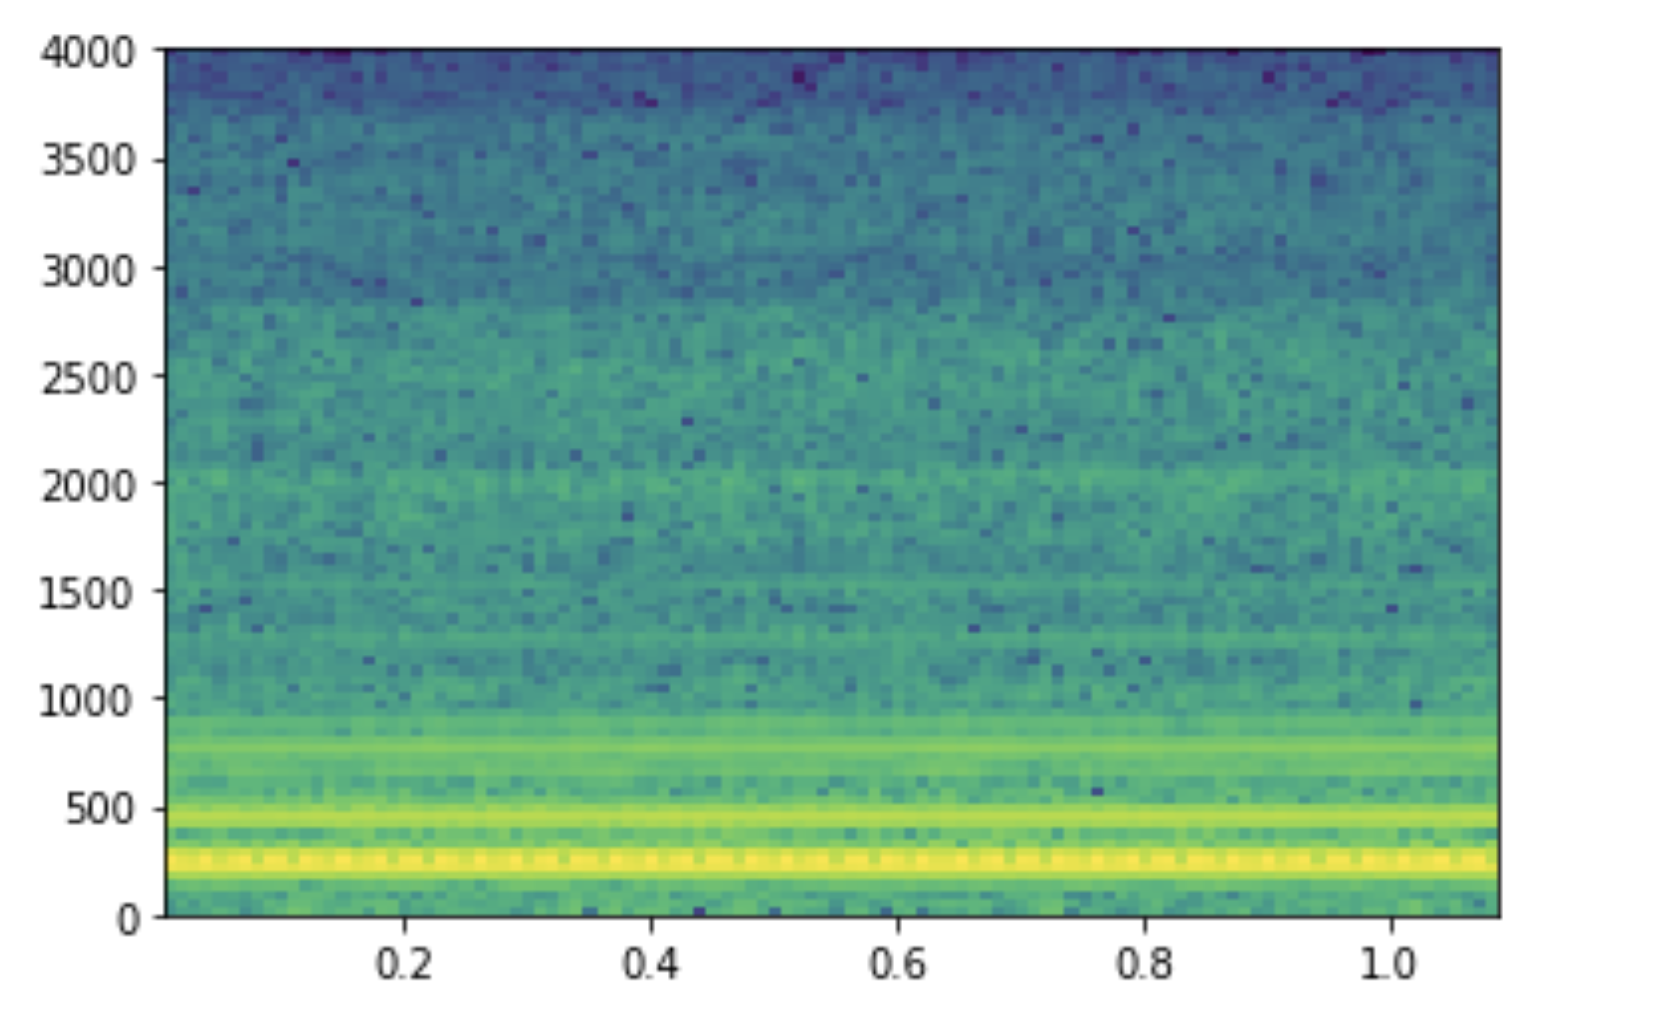
\includegraphics[scale=0.3]{img/spectrogram.png}
\caption{Спектрограмма одной секунды звучания флейты. Разрешение 101 x 549.}
\label{fig:diagram}
\end{figure}

Исходный аудиофайл разбивался на фрагменты длиной в одну секунду, после чего для каждого из них строилась спектрограмма. Все такие спектрограммы подавались на вход нейронной сети, которая по картинке определяла, что за инструмент звучит в данном фрагменте. Архитектура модели была тщательна подобрана, что подтверждается высоким процентом корректных ответов на тестовых данных.

\begin{figure}[H]
\centering
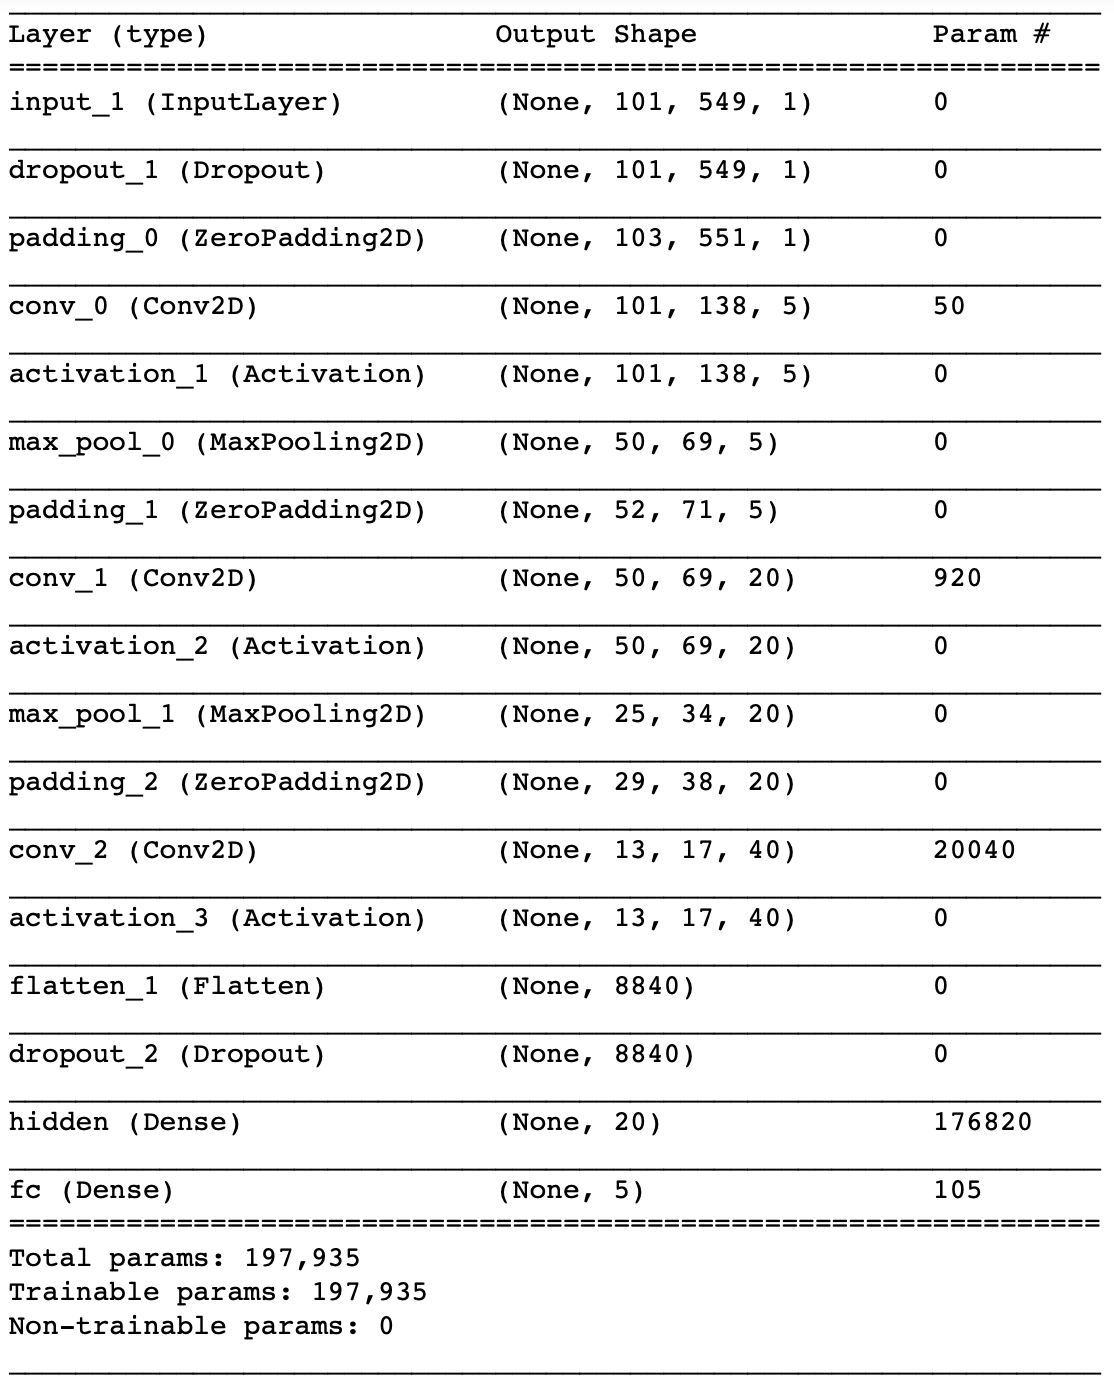
\includegraphics[scale=0.5]{img/model.png}
\caption{Архитектура модели.}
\label{fig:diagram}
\end{figure}

\begin{figure}[H]
\centering
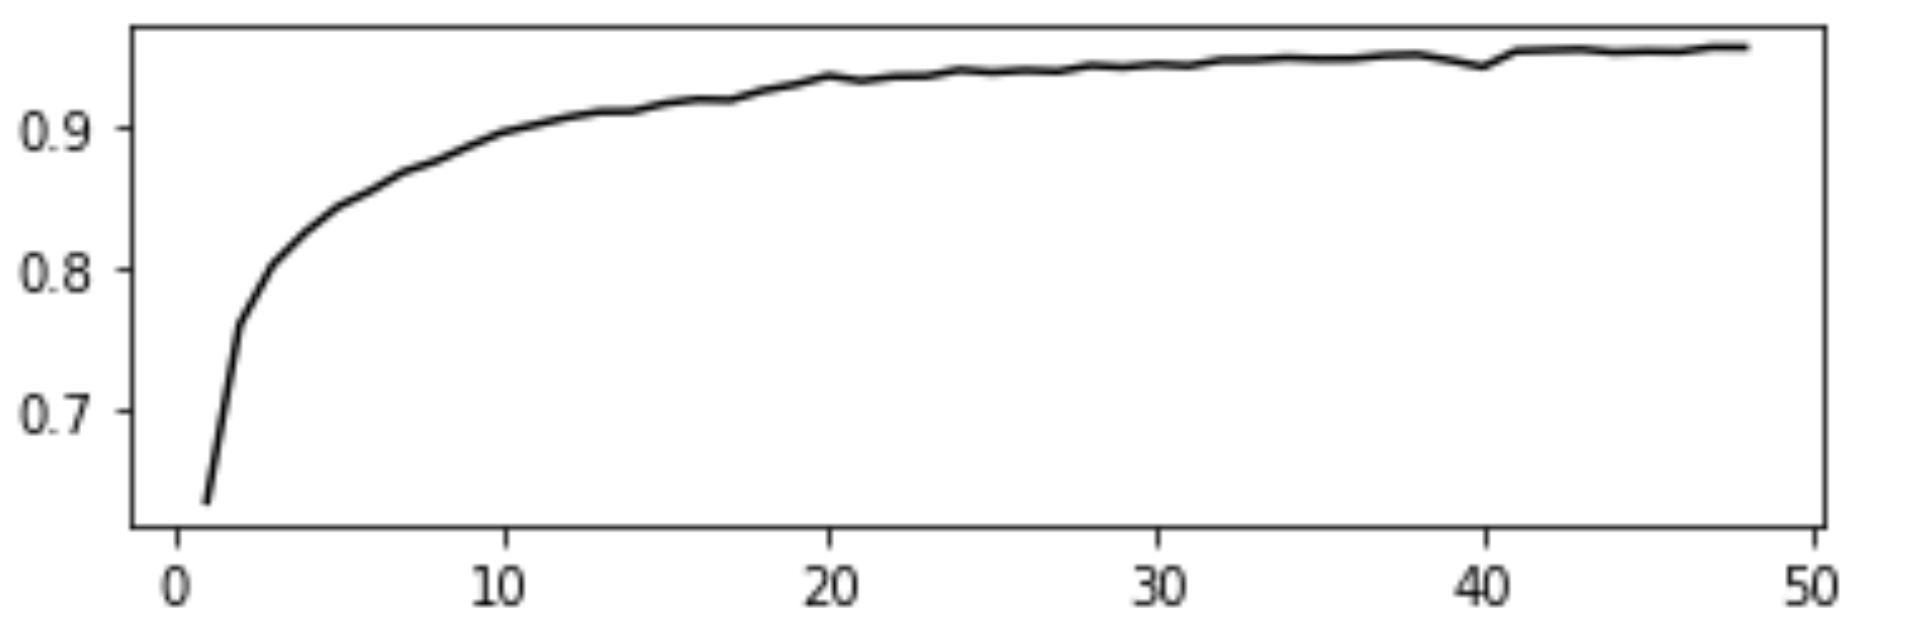
\includegraphics[scale=0.3]{img/training.png}
\caption{Процесс обучения модели. 50 эпох. Достигается точность в 95\%.}
\label{fig:diagram}
\end{figure}

Обучение проводилось на 150 аудиозаписях, скаченных с YouTube. Для каждого из пяти инструментов было скачено по 30 файлов, на каждом из которых инструмент звучал без сопровождения.

Наиболее успешной показала себя модель, архитектура и график обучения которой приведены выше. Модели тестировались на 50 произвольных аудиофайлах (по 10 на каждый инструмент), взятых с того же YouTube.

Как мы видим, на двух записях фортепьяно модель сделала неправильное предсказания. Объяснить это можно тем, что на первой из них у инструмента между молоточками и струнами были вставлены специальные металлические пластинки, делающие звук более гитарным, а на второй представлен некий далёко не идеальный VST-плагин.

В целом, рузультаты обучения можно считать успешными, поскольку были получены рабочие датасет, способ препроцессинга и архитектура модели, а значит эксперимент можно продолжить, используя большее количество инструментов.

\begin{figure}[H]
\centering
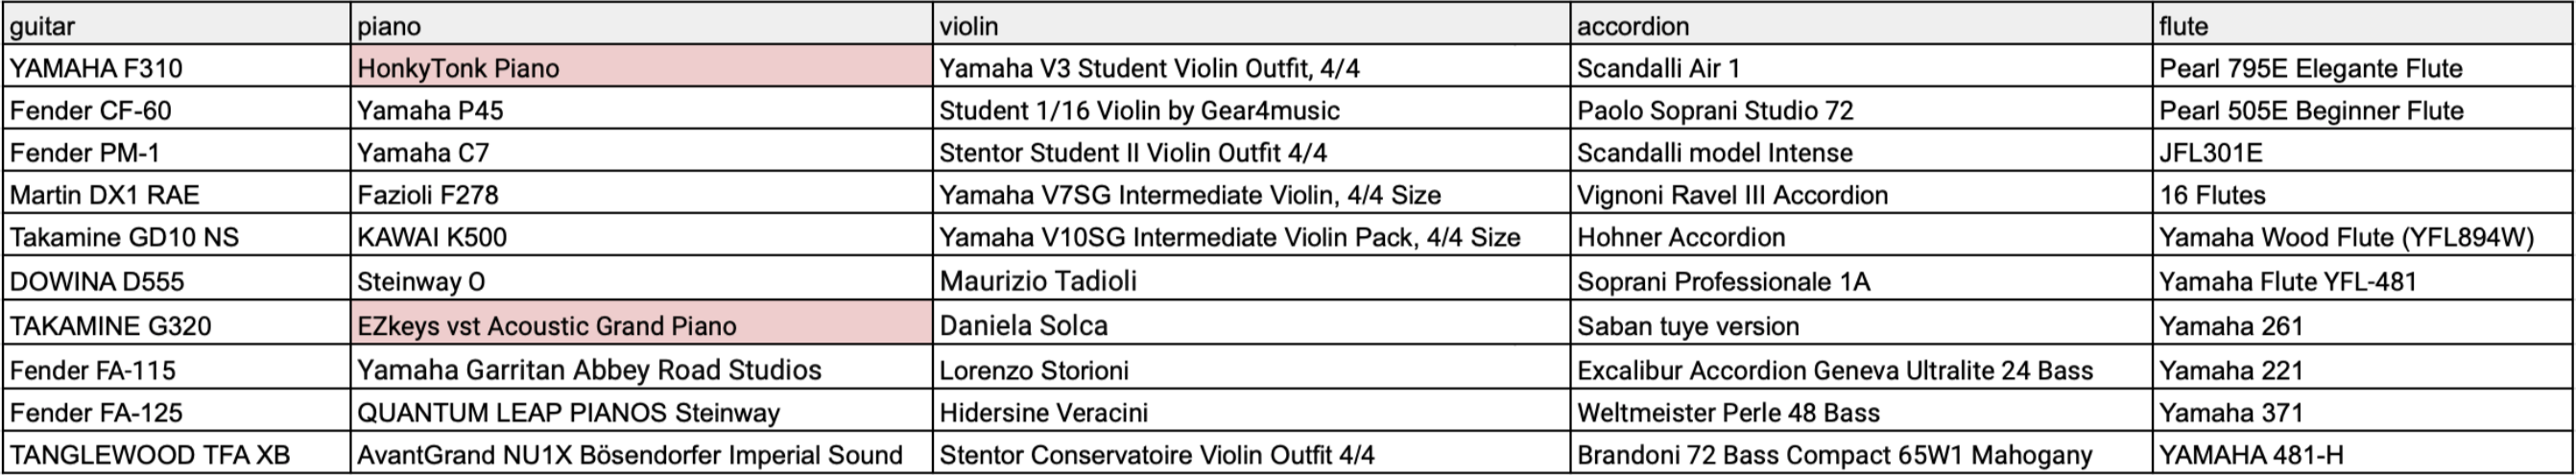
\includegraphics[scale=0.37]{img/results.png}
\caption{Результат работы модели. Красным выделены неправильно угаданные аудиозаписи.}
\label{fig:diagram}
\end{figure}

\subsection{Внутренняя реализация}

После загрузки аудиозаписей на сервер, там происходит побайтовая ''распаковка'' файла (рис. 1). Это позволяет точно определить необходимые для последующей обработки параметры файла.

\begin{figure}[H]
\centering
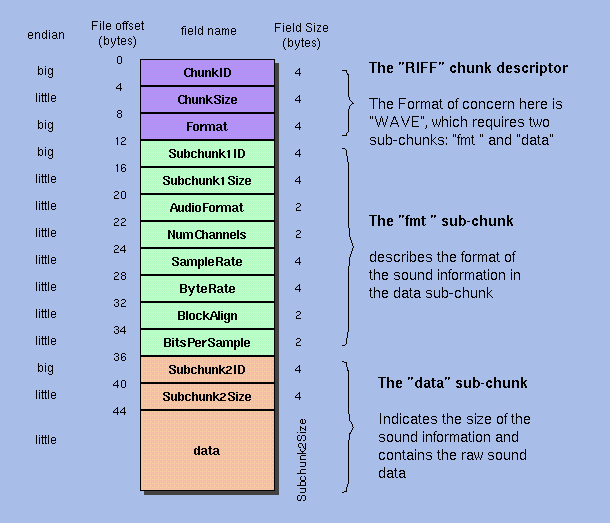
\includegraphics[scale=0.5]{img/wave_format.png}
\caption{Внутренняя структура файла формата WAV.}
\label{fig:wave_format}
\end{figure}

Когда пользователь выбирает функцию, которая подразумевает непосредственную работу с содержимым аудиофайла (например, классификация по музыкальному инструменту или обрезка), то вызывается соответствующая функция расширения PHP. Расширение PHP представляет собой модуль с определенным набором методов, который загружается наравне со встроенными модулями языка PHP. Модуль вызывает метод из скомпилированной заранее библиотеки C++ (использует объектный .so файл). Схематически вызовы изображены на рисунке 2.

\begin{figure}[H]
\centering
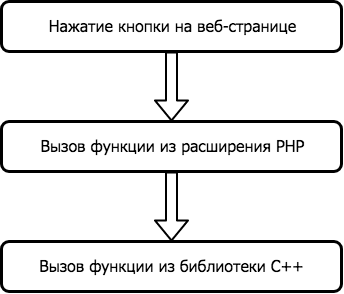
\includegraphics[scale=0.5]{img/diagram.png}
\caption{Схема вызова методов.}
\label{fig:diagram}
\end{figure}

Если выбранная операция является преобразованием аудиофайла, то соответствующий библиотечный метод выполняет это операцию и сохраняет новый файл под другим именем. Если пользователь запросил классификацию аудиозаписи, то на сервере запускается интерпретатор Python3, который получает предсказание заранее обученной нейронной сети. \\

Работа веб-приложения возможна в параллельном режиме, что осуществляется веб-сервером Apache. Для каждой пользовательской сессии извлекается ее уникальный $128$-битный идентификатор сессии, и для каждого такого подключения создается директория, чтобы избегать конфликтов между различными пользователями. Если сессия неактивна в течение определенного времени, то директория сессии на сервере удаляется.

\newpage

\section[Источники]{\huge Источники}

\begin{enumerate}
\item Hojjat Salehinejad, Sharan Sankar: Recent Advances in Recurrent Neural Networks, 2017. \\
URL: https://arxiv.org/abs/1801.01078
\item Asifullah Khan, Anabia Sohail: A Survey of the Recent Architectures of Deep Convolutional Neural Networks, 2019. \\
URL: https://arxiv.org/abs/1901.06032
\item Mingqing Yun, Jing Bi: Deep Learning for Musical Instrument Recognition, 2017
\item Apache HTTP Server Version 2.4 Documentation \\
URL: https://httpd.apache.org/docs/2.4/
\item WAVE PCM soundfile format \\
URL: http://soundfile.sapp.org/doc/WaveFormat/
\item Sara Goleman: Extension Writing Part I: Introduction to PHP and Zend, 2005 \\
URL: https://devzone.zend.com/303/extension-writing-part-i-introduction-to-php-and-zend/
\item Sara Goleman: Extension Writing Part II: Parameters, Arrays, and ZVALs, 2005 \\
URL: https://devzone.zend.com/317/extension-writing-part-ii-parameters-arrays-and-zvals/ \\
URL: https://devzone.zend.com/318/extension-writing-part-ii-parameters-arrays-and-zvals-continued/
\end{enumerate}

\end{document}












